\question (浙江大学,2000年)执行完下列语句段后,i值为( ) int f(int x)\{
return((x\textgreater{}0)?x*f(x-1):2); \} \ldots{}\ldots{} int i=1;
i=f(f(i));
\par\twoch{2}{\textcolor{red}{4}}{8}{无限递归}
\begin{solution}计算过程如下: i=f(f(1))=f(1*f(0))=f(2)=2*f(1)=2*1*f(0)=2*2=4。
\end{solution}
\question (北京航空航天大学,2007年)中缀表达式A-(B+C/D)*E的后缀表形式是( )
\par\twoch{\textcolor{red}{ABCD/+E*-}}{ABC+D/*E-}{AB-C+D/E*}{ABC-+D/E*}
\begin{solution}这个表达式的第一步是计算除法,即C/D,在后缀表达式中,就应该有CD/,四个选项中只有A选项有CD/,因此本题选A。
\end{solution}
\question (江苏大学,2006年)表达式3*2\^{}(4+2*2-6*3)-5求值过程中当扫描到6时,操作数栈和运算符栈为(
),其中\^{}为乘幂,\#表示表达式的开始符
\par\fourch
{3,2,4,1,1,和\#\*\^(+\*\-}
{\textcolor{red}{3,2,8和\#\*\^(\-}}
{3,2,4,2,2和\#\*\^(\-}
{3,2,8和\#\*\^\-}
\begin{solution}扫描到6时,3*2\^{}(4+2*2-6*3)-5中已经计算的为阴影部分。
6之前的计算符有*,\^{},+,*,-,其中4+2*2先计算过了,因此还有*,\^{},-,排除A,D。
6之前的操作数有3,2,4,2,2,又因4+2*2已经先计算过了,因此操作数栈中应为3,2,8,排除C选项,因此本题选B。
\end{solution}
\question (四川大学,2005年)利用栈求表达式的值时,设立操作数栈OPND,设OPND只有两个存储单元,在下列表达式中,不发生上溢的是(
)
\par\twoch{A-B*(C-D)}{\textcolor{red}{(A-B)*C-D}}{(A-B*C)-D}{(A-B)*(C-D)}
\begin{solution}第一种方法将所有表达式转换成后缀表达式再进行判断: A.ABCD-*- B.AB-C*D-
C.ABC*-D- D.AB-CD-* A选项,明显需要4个存储单元。
B选项,只需要2个存储单元。 C选项,明显需要3个存储单元。
D选项,也需要3个存储单元。 综上,本题选B。
第二种方法是按操作优先来判断:
A选项,首先需要进行C-D,而这之前需要存储A、B、C、D,因此需要4个存储单元,排除。
B选项,首先需要进行A-B,只需要存储A、B即可,然后进行(A-B)*C,只需要存储A-B、C即可。最后进行(A-B)*C-D,只需要存储(A-B)*C、D即可,因此需要2个存储单元。
C选项,首先需要进行B*C,这需要存储A、B、C,因此需要3个存储单元,排除。
D选项,首先计算A-B,这需要存储A、B即可,然后进行C-D,这需要存储A-B、C、D,因此需要3个存储单元,排除。
这里给出``中缀表达式→后缀表达式''的人工方法。
比如给出中缀表达式A-B*(C-D),则
1)按照运算符的优先级对所有的运算单位加括号,式子变成了(A-(B*(C-D)))。
2)把运算符号移动到对应的括号后面(如果是转成前缀就移到括号前面),式子变成了(A(B(CD)-)*)-。
3)把括号去掉,式子变成了ABCD-*-。
\end{solution}
\question (上海交通大学,2005年)一个递归过程的定义可以用递归过程求解,也可以用非递归过程求解,但单从运行时间来看,通常递归过程要比非递归过程(
)
\par\twoch{较快}{\textcolor{red}{较慢}}{相同}{无法比较}
\begin{solution}递归调用本身需要使用系统栈,每次分配函数内存以及栈都需要时间。
\end{solution}
\question 若元素a,b,c,d,e,f依次进栈,允许进栈、退栈操作交替进行,但不允许连续三次进行退栈操作,则不可能得到的出栈序列是(
)
\par\twoch{d,c,e,b,f,a}{c,b,d,a,e,f}{b,c,a,e,f,d}{\textcolor{red}{a,f,e,d,c,b}}
\begin{solution}A选项:入栈顺序为:a,b,c,d,e,f。出栈顺序为:d,c,e,b,f,a。
B选项:入栈顺序为:a,b,c,d,e,f。出栈顺序为:c,b,d,a,e,f。
C选项:入栈顺序为:a,b,c,d,e,f。出栈顺序为:b,c,a,e,f,d。
D选项:入栈顺序为:a,b,c,d,e,f。出栈顺序为:a,f,e,d,c,b。按照题设要求,选项D所给序列即为不可能得到的出栈顺序,因为其最后是连续的5个pop(出栈)操作。
\end{solution}
\question 元素a,b,c,d,e依次进入初始为空的栈中,若元素进栈后可停留、可出栈,直到所有的元素都出栈,则在所有可能的出栈序列中,以元素d开头的序列个数是(
)
\par\twoch{3}{\textcolor{red}{4}}{5}{6}
\begin{solution}若要保证出栈序列以d开头,则前3个元素必连续进栈,中间不能出现出栈的情况,然后d出栈,此时栈内元素由底到顶为,a,b,c,栈外元素为e,出栈序列中元素为d。
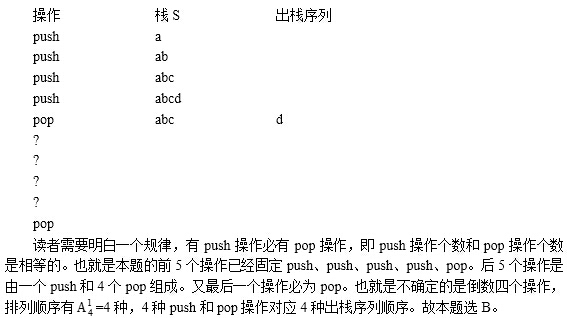
\includegraphics[width=5.90625in,height=3.31250in]{computerassets/e6ce6cda40e4109f129b7eaf9d62c8e2.jpeg}
【总结】
除了根据push和pop操作来确定,本题也可以通过序列的排列顺序来判定,首先a,b,c,d这4个元素在栈内的顺序已定,由栈的先进后出原则,其在出栈序列中的相对位置必为\ldots{}d\ldots{}c\ldots{}b\ldots{}a\ldots{};又因为d的位置已定,所以出栈待定序列必为d\ldots{}c\ldots{}b\ldots{}a\ldots{}。显然在栈外的e可以在任何时候出栈入栈,即可以出现在以上待定序列中任何一个省略号的位置,即出栈序列有4种可能,故选B。
\end{solution}
\question 已知操作符包括``+''、``-''、``*''、``/''、``(''和``)''。将中缀表达式a+b-a*((c+d)/e-f)+g转换为后缀表达式ab+acd+e/f-*-g+时,用栈来存放暂时还不能确定运算次序的操作符。若栈初始时为空,则转换过程中同时保存在栈中的操作符的最大个数是(
)
\par\twoch{\textcolor{red}{5}}{7}{8}{11}
\begin{solution}本题与前三题相比,其实本质上并没有区别,只是把abcde换成了a+b-a*((c+d)/e-f)+g,解法是一模一样的,已知入栈顺序和出栈顺序,求栈操作过程。
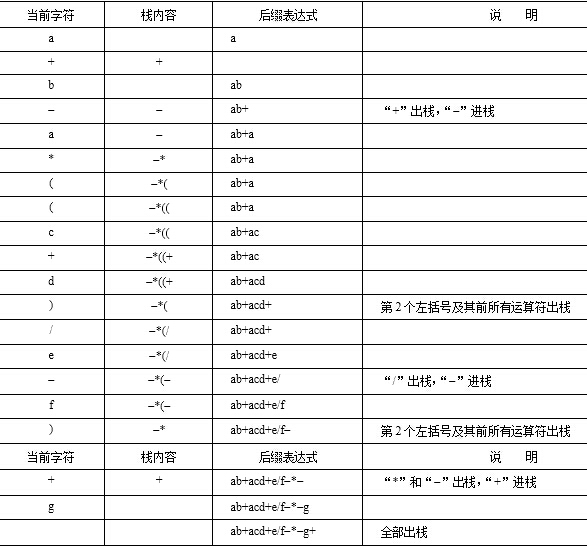
\includegraphics[width=6.11458in,height=5.69792in]{computerassets/c09de64f3ac4b9db2f1a5f93be5d10e5.jpeg}
从中看到栈中最多有5个运算符。故选A。 【总结】
所有的栈相关的题目,都非常类似,基本就是已知入栈和出栈顺序(或部分出栈顺序【11年】)求栈的push、pop操作过程(或可能的栈操作总数【11年】),万变不离其宗。读者只要熟练掌握列表的方法,栈的选择题就都能够正确求解。
\end{solution}
\question 假设栈初始为空,将中缀表达式a/b+(c*d-e*f)/g转化为等价后缀表达式的过程中,当扫描到f时,栈中的元素依次是(
)
\par\twoch{+(*-}{\textcolor{red}{+(-*}}{/+(*-*}{/+-*}
\begin{solution}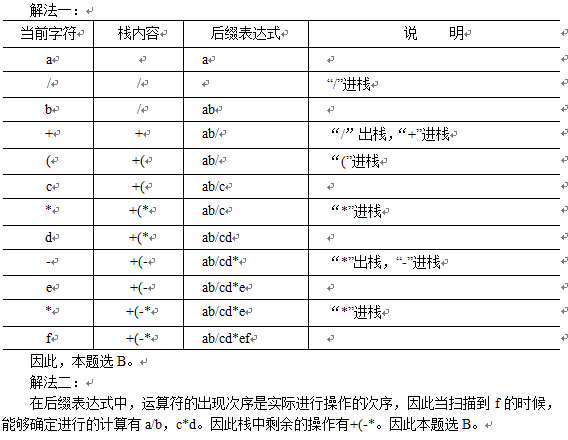
\includegraphics[width=5.91667in,height=4.58333in]{computerassets/22df861753f52f7f3ea6cf28d4a51d95.jpeg}
\end{solution}
\question (青岛大学,2004年)由两个栈共享一个向量空间的好处是( )
\par\fourch{减少存取时间,降低上溢发生的机率}{\textcolor{red}{节省存储空间,降低上溢发生的机率}}{减少存取时间,降低下溢发生的机率}{节省存储空间,降低下溢发生的机率}
\begin{solution}考察共享栈的特点,共享栈是将两个栈的栈顶连接在一起,这样每个栈的栈顶可以自由调配,减少了独立申请时所需要的栈空间,并且当两个栈的指针相遇时,表明共享栈满,不能再入栈了,这样就减少了独立申请栈时可能造成的栈溢出
\end{solution}
\question (浙江大学,2005年)当字符序列t3\_依次入栈,输出长度为3的,且可用做C语言标识符的序列有(
)
\par\twoch{4个}{5个}{\textcolor{red}{3个}}{6个}
\begin{solution}此题当然可以采用枚举法,先找出合法的出栈序列,然后找出符合C语言标识符命名规则的那些序列,但是这样比较麻烦;因为是选择题,我们利用栈的数学性质,我们知道栈的出栈序列的个数满足Cantalan函数,即3个字符的出栈序列的个数一共有5个,另外出去以数字开头的3t\_和3\_t不能作为C语言的标识符外,一共可用的标识符序列共有3个
\end{solution}
\question (重庆大学,2004年)设有一足够大的栈,入栈序列为x,y,z,u,v,下列哪一个出栈序列是不可能的序列(
)
\par\twoch{x,y,z,u,v}{y,x,z,u,v}{\textcolor{red}{z,x,y,u,v}}{v,u,z,y,x}
\begin{solution}由于栈的先进后出规律,在给定的输入序列后,有些输出序列是不可能出现的,比如z,x,y,u,v。因为第一个输出是z,这时x,y一定是已进入栈了。这时栈里面依次是x和y,只可能是y先出,x后出
\end{solution}
\question (北京航空航天大学,2004年)若某堆栈的输入序列为1,2,3\ldots{}\ldots{},n,输出序列的第一个元素为n,则第i个输出元素为(
)
\par\twoch{i}{n-i}{\textcolor{red}{n-i+1}}{哪个元素无所谓}
\begin{solution}每次栈输出后,栈顶元素依次减1,所以第i个元素输出后,栈顶元素为n-i,而输出的元素为n-i+1
\end{solution}
\question (上海交通大学,2005年)一个递归的定义可以用递归过程求解,也可以用非递归过程求解,但单从运行时间来看,通常递归过程要比非递归过程(
)
\par\twoch{较快}{\textcolor{red}{较慢}}{相同}{无法比较}
\begin{solution}递归过程中通常会引入一些元素的反复计算(比如斐波那契数列),而且有堆栈压缩开销,所以通常来说,递归过程要慢于非递归过程。
\end{solution}
